% Options for packages loaded elsewhere
\PassOptionsToPackage{unicode}{hyperref}
\PassOptionsToPackage{hyphens}{url}
%
\documentclass[
]{book}
\usepackage{amsmath,amssymb}
\usepackage{iftex}
\ifPDFTeX
  \usepackage[T1]{fontenc}
  \usepackage[utf8]{inputenc}
  \usepackage{textcomp} % provide euro and other symbols
\else % if luatex or xetex
  \usepackage{unicode-math} % this also loads fontspec
  \defaultfontfeatures{Scale=MatchLowercase}
  \defaultfontfeatures[\rmfamily]{Ligatures=TeX,Scale=1}
\fi
\usepackage{lmodern}
\ifPDFTeX\else
  % xetex/luatex font selection
\fi
% Use upquote if available, for straight quotes in verbatim environments
\IfFileExists{upquote.sty}{\usepackage{upquote}}{}
\IfFileExists{microtype.sty}{% use microtype if available
  \usepackage[]{microtype}
  \UseMicrotypeSet[protrusion]{basicmath} % disable protrusion for tt fonts
}{}
\makeatletter
\@ifundefined{KOMAClassName}{% if non-KOMA class
  \IfFileExists{parskip.sty}{%
    \usepackage{parskip}
  }{% else
    \setlength{\parindent}{0pt}
    \setlength{\parskip}{6pt plus 2pt minus 1pt}}
}{% if KOMA class
  \KOMAoptions{parskip=half}}
\makeatother
\usepackage{xcolor}
\usepackage{color}
\usepackage{fancyvrb}
\newcommand{\VerbBar}{|}
\newcommand{\VERB}{\Verb[commandchars=\\\{\}]}
\DefineVerbatimEnvironment{Highlighting}{Verbatim}{commandchars=\\\{\}}
% Add ',fontsize=\small' for more characters per line
\usepackage{framed}
\definecolor{shadecolor}{RGB}{248,248,248}
\newenvironment{Shaded}{\begin{snugshade}}{\end{snugshade}}
\newcommand{\AlertTok}[1]{\textcolor[rgb]{0.94,0.16,0.16}{#1}}
\newcommand{\AnnotationTok}[1]{\textcolor[rgb]{0.56,0.35,0.01}{\textbf{\textit{#1}}}}
\newcommand{\AttributeTok}[1]{\textcolor[rgb]{0.13,0.29,0.53}{#1}}
\newcommand{\BaseNTok}[1]{\textcolor[rgb]{0.00,0.00,0.81}{#1}}
\newcommand{\BuiltInTok}[1]{#1}
\newcommand{\CharTok}[1]{\textcolor[rgb]{0.31,0.60,0.02}{#1}}
\newcommand{\CommentTok}[1]{\textcolor[rgb]{0.56,0.35,0.01}{\textit{#1}}}
\newcommand{\CommentVarTok}[1]{\textcolor[rgb]{0.56,0.35,0.01}{\textbf{\textit{#1}}}}
\newcommand{\ConstantTok}[1]{\textcolor[rgb]{0.56,0.35,0.01}{#1}}
\newcommand{\ControlFlowTok}[1]{\textcolor[rgb]{0.13,0.29,0.53}{\textbf{#1}}}
\newcommand{\DataTypeTok}[1]{\textcolor[rgb]{0.13,0.29,0.53}{#1}}
\newcommand{\DecValTok}[1]{\textcolor[rgb]{0.00,0.00,0.81}{#1}}
\newcommand{\DocumentationTok}[1]{\textcolor[rgb]{0.56,0.35,0.01}{\textbf{\textit{#1}}}}
\newcommand{\ErrorTok}[1]{\textcolor[rgb]{0.64,0.00,0.00}{\textbf{#1}}}
\newcommand{\ExtensionTok}[1]{#1}
\newcommand{\FloatTok}[1]{\textcolor[rgb]{0.00,0.00,0.81}{#1}}
\newcommand{\FunctionTok}[1]{\textcolor[rgb]{0.13,0.29,0.53}{\textbf{#1}}}
\newcommand{\ImportTok}[1]{#1}
\newcommand{\InformationTok}[1]{\textcolor[rgb]{0.56,0.35,0.01}{\textbf{\textit{#1}}}}
\newcommand{\KeywordTok}[1]{\textcolor[rgb]{0.13,0.29,0.53}{\textbf{#1}}}
\newcommand{\NormalTok}[1]{#1}
\newcommand{\OperatorTok}[1]{\textcolor[rgb]{0.81,0.36,0.00}{\textbf{#1}}}
\newcommand{\OtherTok}[1]{\textcolor[rgb]{0.56,0.35,0.01}{#1}}
\newcommand{\PreprocessorTok}[1]{\textcolor[rgb]{0.56,0.35,0.01}{\textit{#1}}}
\newcommand{\RegionMarkerTok}[1]{#1}
\newcommand{\SpecialCharTok}[1]{\textcolor[rgb]{0.81,0.36,0.00}{\textbf{#1}}}
\newcommand{\SpecialStringTok}[1]{\textcolor[rgb]{0.31,0.60,0.02}{#1}}
\newcommand{\StringTok}[1]{\textcolor[rgb]{0.31,0.60,0.02}{#1}}
\newcommand{\VariableTok}[1]{\textcolor[rgb]{0.00,0.00,0.00}{#1}}
\newcommand{\VerbatimStringTok}[1]{\textcolor[rgb]{0.31,0.60,0.02}{#1}}
\newcommand{\WarningTok}[1]{\textcolor[rgb]{0.56,0.35,0.01}{\textbf{\textit{#1}}}}
\usepackage{longtable,booktabs,array}
\usepackage{calc} % for calculating minipage widths
% Correct order of tables after \paragraph or \subparagraph
\usepackage{etoolbox}
\makeatletter
\patchcmd\longtable{\par}{\if@noskipsec\mbox{}\fi\par}{}{}
\makeatother
% Allow footnotes in longtable head/foot
\IfFileExists{footnotehyper.sty}{\usepackage{footnotehyper}}{\usepackage{footnote}}
\makesavenoteenv{longtable}
\usepackage{graphicx}
\makeatletter
\def\maxwidth{\ifdim\Gin@nat@width>\linewidth\linewidth\else\Gin@nat@width\fi}
\def\maxheight{\ifdim\Gin@nat@height>\textheight\textheight\else\Gin@nat@height\fi}
\makeatother
% Scale images if necessary, so that they will not overflow the page
% margins by default, and it is still possible to overwrite the defaults
% using explicit options in \includegraphics[width, height, ...]{}
\setkeys{Gin}{width=\maxwidth,height=\maxheight,keepaspectratio}
% Set default figure placement to htbp
\makeatletter
\def\fps@figure{htbp}
\makeatother
\setlength{\emergencystretch}{3em} % prevent overfull lines
\providecommand{\tightlist}{%
  \setlength{\itemsep}{0pt}\setlength{\parskip}{0pt}}
\setcounter{secnumdepth}{5}
\usepackage{booktabs}
\usepackage{booktabs}
\usepackage{longtable}
\usepackage{array}
\usepackage{multirow}
\usepackage{wrapfig}
\usepackage{float}
\usepackage{colortbl}
\usepackage{pdflscape}
\usepackage{tabu}
\usepackage{threeparttable}
\usepackage{threeparttablex}
\usepackage[normalem]{ulem}
\usepackage{makecell}
\usepackage{xcolor}
\ifLuaTeX
  \usepackage{selnolig}  % disable illegal ligatures
\fi
\usepackage[]{natbib}
\bibliographystyle{apalike}
\IfFileExists{bookmark.sty}{\usepackage{bookmark}}{\usepackage{hyperref}}
\IfFileExists{xurl.sty}{\usepackage{xurl}}{} % add URL line breaks if available
\urlstyle{same}
\hypersetup{
  pdftitle={Electronic Data Entry Software Options for IEP Surveys},
  pdfauthor={IEP DUWG `e-Device' Sub-group led by Karrin Alstad},
  hidelinks,
  pdfcreator={LaTeX via pandoc}}

\title{Electronic Data Entry Software Options for IEP Surveys}
\author{IEP DUWG `e-Device' Sub-group led by Karrin Alstad}
\date{2023-05-02}

\usepackage{amsthm}
\newtheorem{theorem}{Theorem}[chapter]
\newtheorem{lemma}{Lemma}[chapter]
\newtheorem{corollary}{Corollary}[chapter]
\newtheorem{proposition}{Proposition}[chapter]
\newtheorem{conjecture}{Conjecture}[chapter]
\theoremstyle{definition}
\newtheorem{definition}{Definition}[chapter]
\theoremstyle{definition}
\newtheorem{example}{Example}[chapter]
\theoremstyle{definition}
\newtheorem{exercise}{Exercise}[chapter]
\theoremstyle{definition}
\newtheorem{hypothesis}{Hypothesis}[chapter]
\theoremstyle{remark}
\newtheorem*{remark}{Remark}
\newtheorem*{solution}{Solution}
\begin{document}
\maketitle

{
\setcounter{tocdepth}{1}
\tableofcontents
}
\hypertarget{about}{%
\chapter{About}\label{about}}

This is a \emph{sample} book written in \textbf{Markdown}. You can use anything that Pandoc's Markdown supports; for example, a math equation \(a^2 + b^2 = c^2\).

\hypertarget{usage}{%
\section{Usage}\label{usage}}

Each \textbf{bookdown} chapter is an .Rmd file, and each .Rmd file can contain one (and only one) chapter. A chapter \emph{must} start with a first-level heading: \texttt{\#\ A\ good\ chapter}, and can contain one (and only one) first-level heading.

Use second-level and higher headings within chapters like: \texttt{\#\#\ A\ short\ section} or \texttt{\#\#\#\ An\ even\ shorter\ section}.

The \texttt{index.Rmd} file is required, and is also your first book chapter. It will be the homepage when you render the book.

\hypertarget{render-book}{%
\section{Render book}\label{render-book}}

You can render the HTML version of this example book without changing anything:

\begin{enumerate}
\def\labelenumi{\arabic{enumi}.}
\item
  Find the \textbf{Build} pane in the RStudio IDE, and
\item
  Click on \textbf{Build Book}, then select your output format, or select ``All formats'' if you'd like to use multiple formats from the same book source files.
\end{enumerate}

Or build the book from the R console:

\begin{Shaded}
\begin{Highlighting}[]
\NormalTok{bookdown}\SpecialCharTok{::}\FunctionTok{render\_book}\NormalTok{()}
\end{Highlighting}
\end{Shaded}

To render this example to PDF as a \texttt{bookdown::pdf\_book}, you'll need to install XeLaTeX. You are recommended to install TinyTeX (which includes XeLaTeX): \url{https://yihui.org/tinytex/}.

\hypertarget{preview-book}{%
\section{Preview book}\label{preview-book}}

As you work, you may start a local server to live preview this HTML book. This preview will update as you edit the book when you save individual .Rmd files. You can start the server in a work session by using the RStudio add-in ``Preview book'', or from the R console:

\begin{Shaded}
\begin{Highlighting}[]
\NormalTok{bookdown}\SpecialCharTok{::}\FunctionTok{serve\_book}\NormalTok{()}
\end{Highlighting}
\end{Shaded}

\hypertarget{introduction}{%
\chapter{Introduction}\label{introduction}}

All chapters start with a first-level heading followed by your chapter title, like the line above. There should be only one first-level heading (\texttt{\#}) per .Rmd file.

\hypertarget{e-device-working-group-overview}{%
\section{E-device Working Group Overview}\label{e-device-working-group-overview}}

\hypertarget{goals}{%
\subsection{Goals}\label{goals}}

In general, the goal of the electronic data entry sub-group of the DUWG is to research field data entry software and hardware devices (``e-devices''), and to generate resources that support IEP survey leads in selecting and deploying digital data-entry procedures. This sub-group does not intend to suggest a single solution or software choice for all IEP surveys; rather, the sub-group aims to provide specific application reviews and testing, some methods development, and the start of an IEP e-device users network in effort to facilitate the independent decisions and potential transition of each IEP surveys to electronic data collection methods..

\hypertarget{approach}{%
\subsection{Approach}\label{approach}}

A general approach to the exploration of e-device applications was outlined and agreed on at the initial e-device meetings.

First, an e-device information gathering questionnaire (survey) would be distributed within IEP which specifically collects response data from: 1. Experienced e-device users, 2. Those who are currently researching e-device solutions for their survey applications; and 3. Those who have determined e-devices will not work for them.

Second, following leads from the responses to the survey, this distribution is expanded to include external associates (ICF, NEON, CDFW Marine). Follow-up interviews of the experienced e-device users and vendors are conducted, and demonstrations are arranged for the most promising e-device options.

Third, group members will potentially test specific e-devices apps by making use of free trial licenses, and these trials reported back to the group (SFBS \& Yolo By-pass were early volunteers for trial forms development exercises). Potentially other e-device methods will be researched and developed for demonstration purposes (e.g., collection and integration of external sensor data into e-device applications).

\hypertarget{scope-of-group-activities-and-intended-products}{%
\subsection{Scope of group activities and intended products}\label{scope-of-group-activities-and-intended-products}}

The initial e-device questionnaire was used to identify the most common e-device apps used within IEP (Table 1), the key questions/concerns about using e-devices (section below), as well as the key criteria that will be used to evaluate each software options explored by the working group (Tables 2-7). The main categories considering include options within the forms building tools, including QC related factors such as constrained choices and rules that guide subsequent fields. Other categories include IT security protocols, photo integration, cost of different product options, and factors related to the business model of each vendor, including the longevity of the company and the level/cost of customer/technical support.

\hypertarget{cross}{%
\chapter{E-device Survey}\label{cross}}

An Electronic Field Data-Entry Device (``e-Device'') Survey was distributed to IEP survey leads in July of 2022. The goals of this survey were: 1. To get an understanding of the current level of use of electronic field data entry devices among IEP Survey Staff; 2. To seek information from expert e-device users about both hardware and software considerations, and 3. To the learn specific roadblocks for those who are hesitant to consider shifting to electronic data entry methods.

Three groups were targeted for this survey:\\
1. Experienced e-device users (internal IEP and external agencies),\\
2. IEP Survey Staff who are researching e-devices for field application,\\
3. IEP Survey Staff who don't believe electronic field data collection will work for their application.

\hypertarget{survey-respondents}{%
\section{Survey Respondents}\label{survey-respondents}}

The IEP e-device survey was run for approximately a month and received 24 responses. A link to the original survey and to the compiled survey responses is included in the Appendix 2.

See Figure \ref{fig:survey}.

\begin{figure}

{\centering 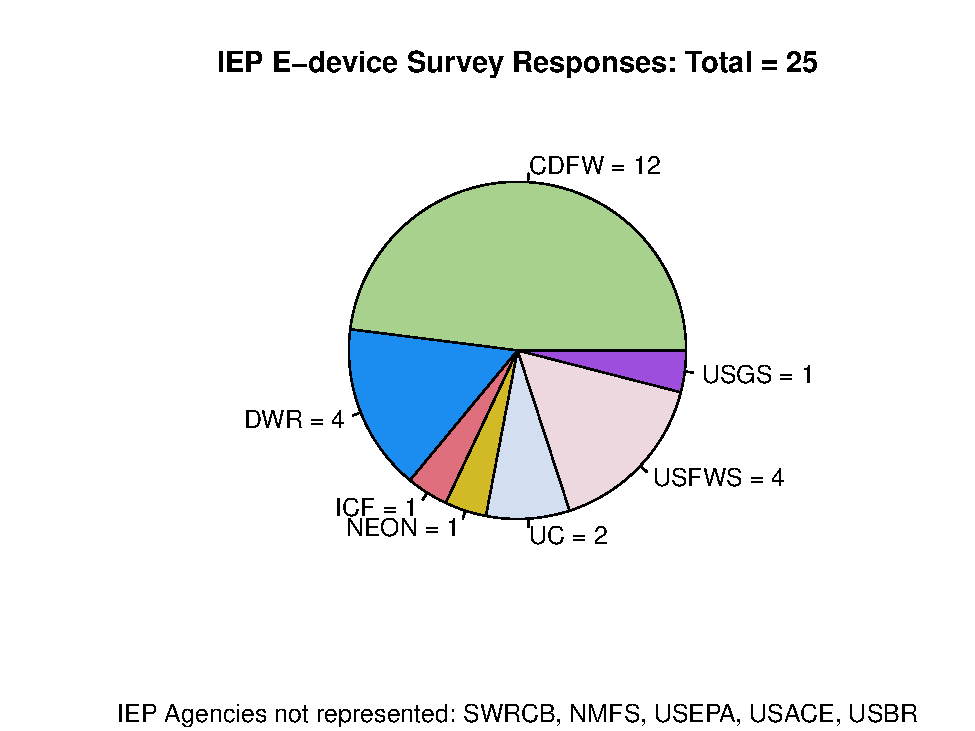
\includegraphics[width=0.8\linewidth]{02-survey_files/figure-latex/survey-1} 

}

\caption{The distribution of of e-device survey responders by agency association. Most of these respondents were CDFW staff, but USFWS and DWR responses were also represented.  Two external agencies (NEON and ICF) were specifically asked to participate after survey responses pointed to these expert resources.}\label{fig:survey}
\end{figure}

Among the 24 respondents, half of these were IEP associates and external contacts that are already using e-device applications for their survey data collections. Five (20\%) of the respondents were IEP associates who were currently seeking e-device solutions for their survey data collections. Two of the respondents indicated that they have already determined that electronic data entry would not work for their IEP survey application, and 5 respondents did not answer the question about their e-device use experience/status. An experienced e-device user resource list has been initiated, including contact names, software type, and type of survey application; this list will be expanded as possible (Appendix ).

\hypertarget{esri-survey123}{%
\chapter{ESRI Survey123}\label{esri-survey123}}

\hypertarget{survey123-overview}{%
\section{Survey123 Overview}\label{survey123-overview}}

From ESRI documentation: ArcGIS Survey123 is a complete, form-centric solution for creating, sharing, and analyzing surveys. Use it to create forms with skip logic, defaults, and support for multiple languages. Collect data using web or mobile devices, even when disconnected from the internet. Upload data securely, and analyze results on the web or in an ArcGIS app.
\url{https://doc.arcgis.com/en/survey123/reference/whatissurvey123.htm}

From G2 Business Software Review: Survey123 is included with ArcGIS, and provides powerful features to help you leverage the power of location to boost your productivity while capturing data and analyzing the results of your surveys. \url{https://www.g2.com/products/arcgis-survey123/reviews}

\hypertarget{survey123-forms-options}{%
\section{Survey123 Forms Options}\label{survey123-forms-options}}

Surveys123 Survey Forms are created and stored through the ESRI web interface (see Figure 1); access requires a current ESRI license. Survey123 forms can be downloaded to tablets, iPhones or iPads, and data collection can be made while the device is offline. Survey results are uploaded to cloud storage next time the device is on-line.

\begin{figure}
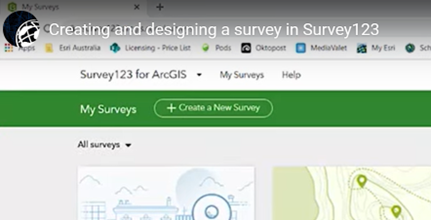
\includegraphics[width=0.9\linewidth]{figures/survey123/ESRIweb} \caption{Screen capture of the ESRI web interface for Survey123 and the option to Create New Survey.}\label{fig:ESRIweb}
\end{figure}

There are two main options for designing a Survey123 survey form: the Web Designer or Survey123 Connect tool. The Web Designer is a web-based menu-driven GUI that does not require learning any specific coding to set up a basic survey form. Survey questions and response types can be specified using a drag and drop tool.

\begin{figure}
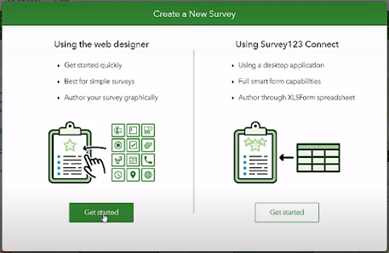
\includegraphics[width=0.9\linewidth]{figures/survey123/ESRIweb2} \caption{Screen capture of the ESRI web interface for Survey123 highlighting the two main options for designing a Survey123 form: the web designer or the Survey123 Connect tool.}\label{fig:ESRIweb2}
\end{figure}

Survey123 Connect is an option for more advanced survey form design, such as a nested structure or calculated responses using user inputs. The Survey123 Connect approach requires defining the more advanced form properties within an `XLSForm spreadsheet' using the XLSForm coding language. ESRI documentation for both Web designer and Connect can be found at: \url{https://doc.arcgis.com/en/survey123/browser/create-surveys/createsurveys.htm}
XLSForm formatting language is described at: \url{https://xlsform.org/en/}.

\begin{figure}
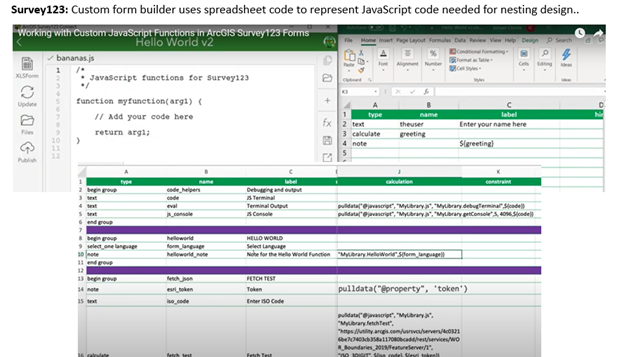
\includegraphics[width=0.9\linewidth]{figures/survey123/survey123_xlsform} \caption{Screen capture of ESRI Survey123 Connect software demonstrating the use of the XLSForm spreadsheet-based coding language and the ability to directly edit the JavaScript code that is linked to XLSForm parameters.}\label{fig:xlsform}
\end{figure}

\begin{figure}
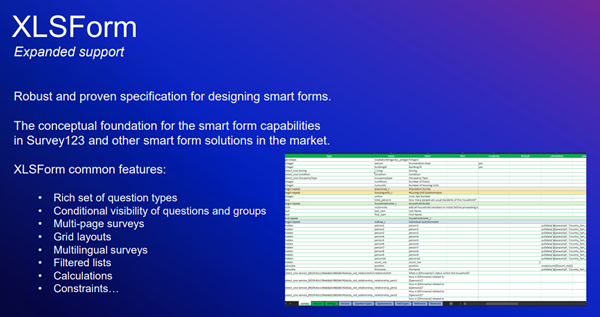
\includegraphics[width=0.9\linewidth]{figures/survey123/survey123_xlsform2} \caption{Screen capture of ArcGIS website description of the XLSForm features: https://gis.idaho.gov/wp-content/uploads/2021/03/ArcGIS-Apps-for-the-Field-State-of-ID.pdf.}\label{fig:xlsform2}
\end{figure}

\begin{longtable}[t]{lllllrl}
\caption{\label{tab:forms123} Survey123 Forms Options}\\
\toprule
\multicolumn{3}{c}{Forms Options} & \multicolumn{4}{c}{ } \\
\cmidrule(l{3pt}r{3pt}){1-3}
Feature & Available & Description & Group Notes/Reviews/ Questions & External Reviews & Score (0-3) & QC\\
\midrule
Geo-referencing & Yes & Every Survey123 entry (object?) has an associated lat/long data & Uses device navigation: phone app or GPS device; Data can open in data in ArcGIS maps directly; Can change base map; Default is current location; Can tap the map to change location  

https://doc.arcgis.com/en/survey123/browser/analyze-results/viewresults.htm\#:\textasciitilde{}:text=Under\%20the\%20title\%20for\%20your,geodatabase)\%20and\%20download\%20your\%20data & NA & 3 & NA\\
Off-line capacity & Yes & Field App works offline and online & Does the data uploads automatically when back on-line?? & NA & NA & NA\\
Ease of Form Development & NA & NA & NA & NA & NA & NA\\
Intuitive form design tool & Yes & Web designer & Web designer intuitive & NA & NA & NA\\
NA & No & Survey123 Connect: XLSForm spreadsheet & XLSForm formatting language required some effort to pick up. & NA & 1 & NA\\
\addlinespace
Coding language required? & No & Web designer & Web designer is a GUI tool that is menu driven and does not require learning any coding & NA & NA & NA\\
NA & Yes & XLSForm spreadsheet & Web designer is a GUI tool that is menu driven and does not require learning any coding & NA & NA & NA\\
NA & NA & Survey123 Connect: XLSForm spreadsheet & Survey123 Connect is an option for more advanced survey designs which requires configuration of an ‘XLSForm spreadsheet’.  XLSForm is an ESRII coding language specific to forms configuration. & Can be hard to edit XLSForm code: 
“Per my experience, if I delete some of the questions and add other [using] filters for the answers through the [XLSForm spread sheet], the answers will be totally. So, every time I have to make a new form for every survey in order to avoid messy information.” https://www.g2.com/products/arcgis-survey123/reviews\#survey-response-2728634

“If you make a change to the form after is has been published it is hard to get the new changes without deleting any previously gathered data.”
https://www.g2.com/products/arcgis-survey123/reviews?page=2 & NA & NA\\
Form Logic and Validation & NA & NA & NA & NA & NA & NA\\
Constrained choices & Yes & Web Designer & -Restricted lengths, Default values (e.g., Date, Time from device) & NA & NA & NA\\
\addlinespace
NA & Yes & Survey123 Connect: XLSForm spreadsheet & Above functionality, plus more advanced options such as: - select multiple responses from a list;smart fields: expressions and formulas to control the allowable input (e.g., total percentage <= 100\%)
- Auto limit by partial input
- Auto-completed suggestion & NA & NA & NA\\
Rules guiding answer series (e.g., “Conditional Questions” and “Skips”) & Yes & Web Designer  & This can be done with Web Designer using the ‘Set rule function’; However, in Web Designer, this function is limited to Single choice, Dropdown, 
Likert scale, and Rating questions & https://support.esri.com/en/technical-article/000022942 & NA & NA\\
NA & Yes & Survey123 Connect: XLSForm spreadsheet & NA & NA & NA & NA\\
Form Look and Feel & NA & NA & NA & NA & NA & NA\\
Flexibility to configure in a logical order for field entry & No & Web Designer  & NA & NA & NA & NA\\
\addlinespace
NA & Yes & Survey123 Connect: XLSForm spreadsheet & In trial demo (Appendix 3): The XLSForm coding was required to represent a nested sampling design; this effort was time consuming to optimize & NA & NA & NA\\
Different styles of question types & Yes & Web Designer  & Yes, both Web designer and Connect provide a range of question types: & https://doc.arcgis.com/en/survey123/browser/create-surveys/webdesigneressentials.htm & NA & NA\\
NA & Yes & Survey123 Connect: XLSForm spreadsheet & NA & NA & NA & NA\\
Form Storage and Permissions Management & Yes & NA & NA & NA & NA & NA\\
Muti-users of an app & Yes & More than one user can submit data to an app at a time (same database); Survey123 HUB: can review responses by user & NA & NA & NA & NA\\
\addlinespace
Real-time Data Review & Yes & Survey123 HUB & The HUB webbased tool allows one to review raw data and summarize data submitted to each survey in the ‘Data’ and ‘Analyze’ tabs; Other summaries: word clouds, frequency plots & NA & NA & NA\\
NA & No & Survey123 Connect & In trial demo, it was difficult to produce a listing of the lengths which was needed for field QC & NA & NA & NA\\
Real-time Edit (“on the fly”) & Yes & User needs to open a separate tab to edit the responses & NA & NA & NA & NA\\
Multiple-language options & Yes & Form can be transposed to other languages; language of stored responses can be specified. & NA & NA & NA & NA\\
\bottomrule
\end{longtable}

\hypertarget{footnotes-and-citations}{%
\chapter{Footnotes and citations}\label{footnotes-and-citations}}

\hypertarget{footnotes}{%
\section{Footnotes}\label{footnotes}}

Footnotes are put inside the square brackets after a caret \texttt{\^{}{[}{]}}. Like this one \footnote{This is a footnote.}.

\hypertarget{citations}{%
\section{Citations}\label{citations}}

Reference items in your bibliography file(s) using \texttt{@key}.

For example, we are using the \textbf{bookdown} package \citep{R-bookdown} (check out the last code chunk in index.Rmd to see how this citation key was added) in this sample book, which was built on top of R Markdown and \textbf{knitr} \citep{xie2015} (this citation was added manually in an external file book.bib).
Note that the \texttt{.bib} files need to be listed in the index.Rmd with the YAML \texttt{bibliography} key.

The \texttt{bs4\_book} theme makes footnotes appear inline when you click on them. In this example book, we added \texttt{csl:\ chicago-fullnote-bibliography.csl} to the \texttt{index.Rmd} YAML, and include the \texttt{.csl} file. To download a new style, we recommend: \url{https://www.zotero.org/styles/}

The RStudio Visual Markdown Editor can also make it easier to insert citations: \url{https://rstudio.github.io/visual-markdown-editing/\#/citations}

\hypertarget{blocks}{%
\chapter{Blocks}\label{blocks}}

\hypertarget{equations}{%
\section{Equations}\label{equations}}

Here is an equation.

\begin{equation} 
  f\left(k\right) = \binom{n}{k} p^k\left(1-p\right)^{n-k}
  \label{eq:binom}
\end{equation}

You may refer to using \texttt{\textbackslash{}@ref(eq:binom)}, like see Equation \eqref{eq:binom}.

\hypertarget{theorems-and-proofs}{%
\section{Theorems and proofs}\label{theorems-and-proofs}}

Labeled theorems can be referenced in text using \texttt{\textbackslash{}@ref(thm:tri)}, for example, check out this smart theorem \ref{thm:tri}.

\begin{theorem}
\protect\hypertarget{thm:tri}{}\label{thm:tri}For a right triangle, if \(c\) denotes the \emph{length} of the hypotenuse
and \(a\) and \(b\) denote the lengths of the \textbf{other} two sides, we have
\[a^2 + b^2 = c^2\]
\end{theorem}

Read more here \url{https://bookdown.org/yihui/bookdown/markdown-extensions-by-bookdown.html}.

\hypertarget{callout-blocks}{%
\section{Callout blocks}\label{callout-blocks}}

The \texttt{bs4\_book} theme also includes special callout blocks, like this \texttt{.rmdnote}.

You can use \textbf{markdown} inside a block.

\begin{Shaded}
\begin{Highlighting}[]
\FunctionTok{head}\NormalTok{(beaver1, }\AttributeTok{n =} \DecValTok{5}\NormalTok{)}
\CommentTok{\#\textgreater{}   day time  temp activ}
\CommentTok{\#\textgreater{} 1 346  840 36.33     0}
\CommentTok{\#\textgreater{} 2 346  850 36.34     0}
\CommentTok{\#\textgreater{} 3 346  900 36.35     0}
\CommentTok{\#\textgreater{} 4 346  910 36.42     0}
\CommentTok{\#\textgreater{} 5 346  920 36.55     0}
\end{Highlighting}
\end{Shaded}

It is up to the user to define the appearance of these blocks for LaTeX output.

You may also use: \texttt{.rmdcaution}, \texttt{.rmdimportant}, \texttt{.rmdtip}, or \texttt{.rmdwarning} as the block name.

The R Markdown Cookbook provides more help on how to use custom blocks to design your own callouts: \url{https://bookdown.org/yihui/rmarkdown-cookbook/custom-blocks.html}

\hypertarget{sharing-your-book}{%
\chapter{Sharing your book}\label{sharing-your-book}}

\hypertarget{publishing}{%
\section{Publishing}\label{publishing}}

HTML books can be published online, see: \url{https://bookdown.org/yihui/bookdown/publishing.html}

\hypertarget{pages}{%
\section{404 pages}\label{pages}}

By default, users will be directed to a 404 page if they try to access a webpage that cannot be found. If you'd like to customize your 404 page instead of using the default, you may add either a \texttt{\_404.Rmd} or \texttt{\_404.md} file to your project root and use code and/or Markdown syntax.

\hypertarget{metadata-for-sharing}{%
\section{Metadata for sharing}\label{metadata-for-sharing}}

Bookdown HTML books will provide HTML metadata for social sharing on platforms like Twitter, Facebook, and LinkedIn, using information you provide in the \texttt{index.Rmd} YAML. To setup, set the \texttt{url} for your book and the path to your \texttt{cover-image} file. Your book's \texttt{title} and \texttt{description} are also used.

This \texttt{bs4\_book} provides enhanced metadata for social sharing, so that each chapter shared will have a unique description, auto-generated based on the content.

Specify your book's source repository on GitHub as the \texttt{repo} in the \texttt{\_output.yml} file, which allows users to view each chapter's source file or suggest an edit. Read more about the features of this output format here:

\url{https://pkgs.rstudio.com/bookdown/reference/bs4_book.html}

Or use:

\begin{Shaded}
\begin{Highlighting}[]
\NormalTok{?bookdown}\SpecialCharTok{::}\NormalTok{bs4\_book}
\end{Highlighting}
\end{Shaded}


  \bibliography{book.bib,packages.bib}

\end{document}
